\documentclass[grey,handout]{beamer}
%\usetheme{Pittsburgh}
\usetheme{Montpellier}
\usepackage{amsmath}
\usepackage{graphicx}
\usepackage{multicol}

\renewcommand{\frametitle}[1]{\begin{center}\textbf{#1}\end{center}}

\def\dd{{\rm d}}
\def\E{\mathbb{E}}
\def\BigO{{\cal O}}

\begin{document}
\title{Numerical Comparative Statics in a Dynamic System: Ball Python Breeding}

\author{Donald M.~DiJacklin}
\date{17 June 2018}

\begin{frame}
  \titlepage
\end{frame}

\begin{frame}
\frametitle{ROADMAP OF SEMINAR}
  \begin{enumerate}[<+->]
    \item Observations
    \item Assumptions
    \item Theory
    \item Some Preliminary Results
  \end{enumerate}
\end{frame}


\begin{frame}
\frametitle{Observations}
  \begin{enumerate}[<+->]
    \item If you're not intending to breed a snake, sell immediately.
    \item Males can inseminate 5 females apiece.
    \item About 60\% of pairings result in a `clutch'.
    \item It costs about \$80 to keep a snake for a year.
    \item A male takes a year to grow to a breedable size.
    \item A female takes two years.
  \end{enumerate}
  

\end{frame}
\begin{frame}
  \frametitle{Assumptions}
  \begin{enumerate}
    \item Clutch size is distributed discrete triangular [2,13] max 6.
    \item A breeder has a capacity that they are not willing to exceed.
    \item No sickness.
  \end{enumerate}
\end{frame}

\begin{frame}
  \frametitle{Theory}
  \begin{itemize}
    \item PAM (with a caveat)
    \begin{align*}
      \max_{\mathbf{x},\mathbf{y},\mathbf{z}}\{ &\mathbf 1_I^T\mathbf R^T\mathbf{x}\mathbf 1_J - 80\mathbf y^T\mathbf 1_I - 80\mathbf z^T\mathbf 1_J \}\\
      s.t. \quad& \mathbf x\mathbf 1_J \leq 5\mathbf 1_I \\
      & \mathbf x^T \mathbf 1_I \leq \mathbf1_J\\
      & \mathbf x \mathbf1_J\leq M\mathbf y\\
      & \mathbf x^T\mathbf 1_I \leq M\mathbf z\\
      & \mathbf y^T\mathbf 1_I + \mathbf z^T\mathbf 1_J \leq 15\\
      & x_{ij}, y_i, z_j \in \{0,1\}
    \end{align*}
  \end{itemize}
\end{frame}


\begin{frame}
  \frametitle{Preliminary Results}
  \begin{multicols}{2}
    \begin{figure}[H]
    \centering
    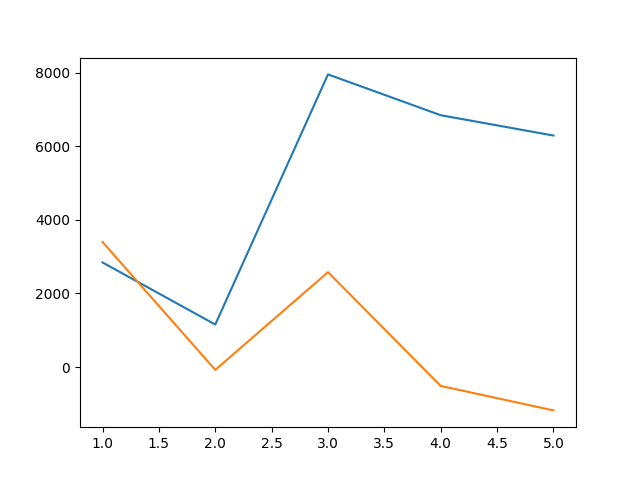
\includegraphics[width=.5\textwidth]{Figure_1.png}
    \end{figure}
    
    \begin{figure}[H]
    \centering
    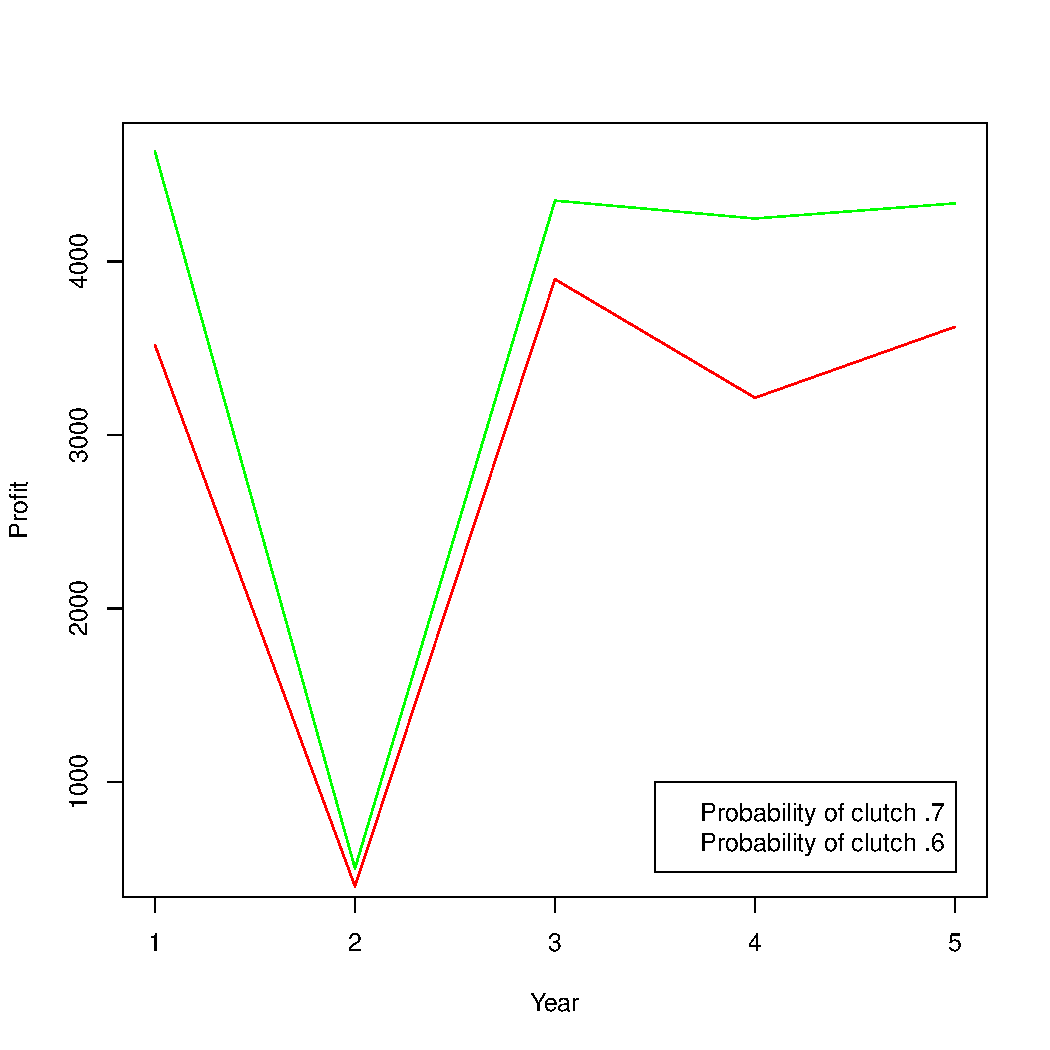
\includegraphics[width=.5\textwidth]{prelimcompstat.pdf}
    \end{figure}
    \end{multicols}

\end{frame}



\end{document}